\begingroup
\renewcommand{\cleardoublepage}{}
\renewcommand{\clearpage}{}
\chapter{Communications cloud}
\endgroup

Pour commencer, il est primordial de rappeler que la plupart du temps, les services du cloud sont accessibles par les utilisateurs via Internet \cite{internet_cloud}. Le protocole IP et ses mécanismes sont utilisés pour permettre la communication entre l'utilisateur et le cloud \cite{use_ip_cloud} afin de délivrer les services du cloud et assurer l'échange de données.

\section{Communications inter-cloud}\label{sec:inter_cloud}

Les communications inter-cloud sont similaires aux autres communications sur Internet et posent les mêmes problématiques en terme de sécurité. Ces problèmes de sécurité interviennent au plus haut de la couche à la plus basse de la pile \gls{TCP/IP} et chacune ajoute de l'information dans les paquets envoyés. Heureusement, des solutions existent et la sécurité est présente dans plusieurs couches du modèle TCP/IP. Toutefois, il n'est pas toujours nécessaire de crypter et sécuriser chaque couche.

\begin{description}
	\item[Couche application :] utilise des mécanismes de sécurité pour une application donnée, séparés des autres couches. \textit{Pretty Good Privacy} (PGP) \cite{pgp} est un exemple d'utilisation sur la couche application. L'envoi de courrier électronique sécurisés est possible grâce aux fonctionnalités de PGP : chiffrer des textes et les signer.  
	\item[Couche transport :] des contrôles de sécurité permettent de protéger les données en transit entre deux hôtes distants. \textit{Transport Layer Security} \cite{tls} et \textit{Secure Sockets Layer} \cite{ssl} sont des protocoles cryptographiques permettent de sécuriser les échanges sur Internet via la couche transport. Ils permettent l'authentification de l'hôte distant et la confidentialité et l'intégrité des données échangées. Des modifications peuvent être nécessaire à certaines applications pour utiliser ces protocoles. 
	\item[Couche réseau :] toutes les communications entre deux hôtes ou avec le réseau peuvent être protégées avec cette couche sans modification spécifique. IPSec \cite{ip_security} est un ensemble de protocoles utilisant des algorithmes garantissant des échanges sécurisés en authentifiant et chiffrant chaque paquet entre deux hôtes distants.
\end{description}

La sécurité au niveau de la couche réseau est la solution la plus souvent utilisée pour protéger l'ensemble des applications et les informations IP. IPSec est utilisé majoritairement pour fournir un \textit{Virtual Private Networking} (VPN) \cite{ipsec_vpn}, plus précisément un VPN site-à-site. Un VPN est un réseau privé virtuel, construit sur un réseau physique existant et fournissant un lien direct entre deux hôtes distants et offrant un échange de données sécurisé. En effet, en isolant le trafic entre les deux hôtes distants, un VPN facilite la sécurité de la communication  sur des réseaux publics. Un VPN site-à-site permet d'établir plusieurs connexions sécurisés avec plusieurs hôtes situés à différentes locations entre eux afin de former un groupe d'utilisateurs fermés, appelé \textit{Closed User Group} (CUG). Aujourd'hui, via le service IPSecVPN, les connexions inter-cloud permettent d'offrir des garanties de sécurité satisfaisantes. Cependant, le nombre d'utilisateurs se connectant aux CSP va augmenter considérablement et vont, sans doute, utiliser plusieurs services de cloud différents. Ainsi, le nombre de réseaux clouds connectés via IPSec VPN va augmenter considérablement également. Il est nécessaire donc de proposer une solution durable et performante basé sur IPSecVPN.

\begin{figure}[h]
	\center
	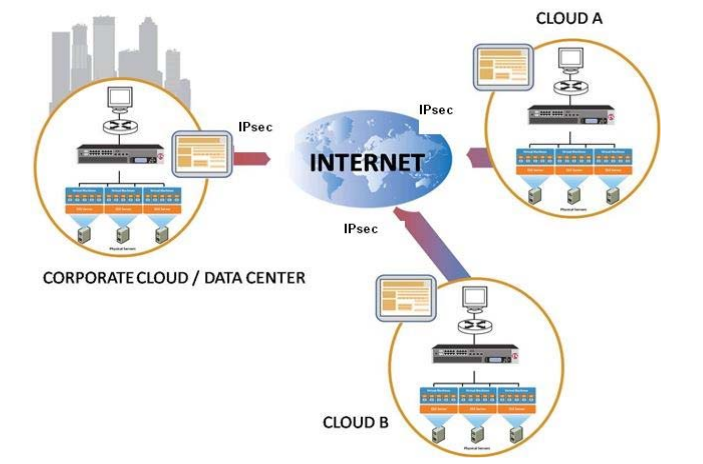
\includegraphics[height=5.5cm]{./pics/inter_cloud_archi_general.png}
	\caption{Architecture général des communications inter-cloud \cite{archi_inter}}
	\label{label-image3}
\end{figure}

Dayananda M. S. et Ashwin K. proposent une architecture pour les communications inter-cloud utilisant IPSecVPN \cite{archi_inter}. Il existe deux types d'architecture IPSecVPN principales : \textit{Full Mesh} et \textit{Hub-and-Spoke}. L'architecture \textit{Full Mesh} se caractérise par une connections de tous les réseaux entre eux et les réseaux vont communiqués en utilisant IPSec. L'architecture \textit{Hub-and-Spoke} est le modèle le plus utilisé avec un \textit{hub} placé entre tous les réseaux et les connectant. Un seul lien IPSec est nécessaire, c'est le lien entre le réseau et le \textit{hub}.
Les deux architectures présentent chacune des problèmes de performance, par exemple, lorsque le nombre de CUG augmente ou encore lorsque le trafic entre les CUG augmente. Pour résoudre le problème de performance, il se base sur l'architecture textit{Hub-and-Spoke} afin de mettre en place un système de IPSecVPN qui créer dynamiquement les tunnels entre les différents clouds en fonction de la demande.
\newline
L'architecture proposée permet tout d'abord d'établir des connexions IPSec dynamiques via des accès VPN multi-points en combinant le chiffrement d'IPSec, des tunnels \textit{Generic Routing Encapsulation} (\gls{GRE}) et le protocole \textit{Next Hop Resolution} (\gls{NHRP}). Il est nécessaire que chaque routeur (autre que le \textit{Hub}) possède une interface point-à-point afin de pouvoir créer le tunnel vers le \textit{Hub}. On oblige alors tout le trafic entre les routeurs, appelé \textit{Spoke}, a transité par le \textit{Hub}. De plus, si un \textit{Spoke} transmet des données, le \textit{Hub} agit alors comme serveur NHRP afin de déterminer dynamiquement l'adresse de destination. Il est à noter que lorsque le \textit{Hub} agit comme serveur NHRP, il permet à GRE de configurer et déterminer les adresses de destination les plus courtes des autres pairs. Les deux routeurs, source et destination, vont alors lancer IPSec entre eux et ainsi créer dynamiquement un tunnel GRE point-à-point, mais également commencer les négociations des sessions IPSec directement sans configuration traditionnelle (gain de temps considérable). Ce tunnel sera automatiquement tombé après une certaine période d'activité. Ensuite, autre avantage de ce type de configuration est que les \textit{Spoke} peuvent utiliser une adresse IP dynamique, car NHRP permet de déterminer l'adresse IP de l'interface du \textit{Spoke} distant via le routeur \textit{Hub}. Enfin, dernier avantage, la configuration du \textit{Hub} est grandement simplifiée puisqu'elle n'a pas besoin de configurer les informations GRE ou IPSec des \textit{Spoke}, car elles sont apprises dynamiquement via NHRP. De plus, la configuration permet d'ajouter un nouveau \textit{Spoke} sans configuration supplémentaire, car ce dernier va s'enregistrer auprès du \textit{Hub} dynamiquement et les différentes informations du nouveau \textit{Spoke} seront propagées vers les autres pairs et inversement. Pour finir, l'architecture proposée, sur la figure \ref{label-image4}, apporte également une autre fonctionnalité : lorsqu'une nouvelle connexion IPSec/IKE est établie entre deux \textit{Spoke}, les règles de filtrage de \textit{Hub} ne sont pas appliqués entre eux. L'utilisation d'une extension du \textit{Traffic Selector} (TS) permet de placer les différents filtres dans la création de la session IPSec/IKE afin d'établir les règles de filtrage dans l'échange IPSec/IKE entre les deux \textit{Spoke}.

\begin{figure}[h]
	\center
	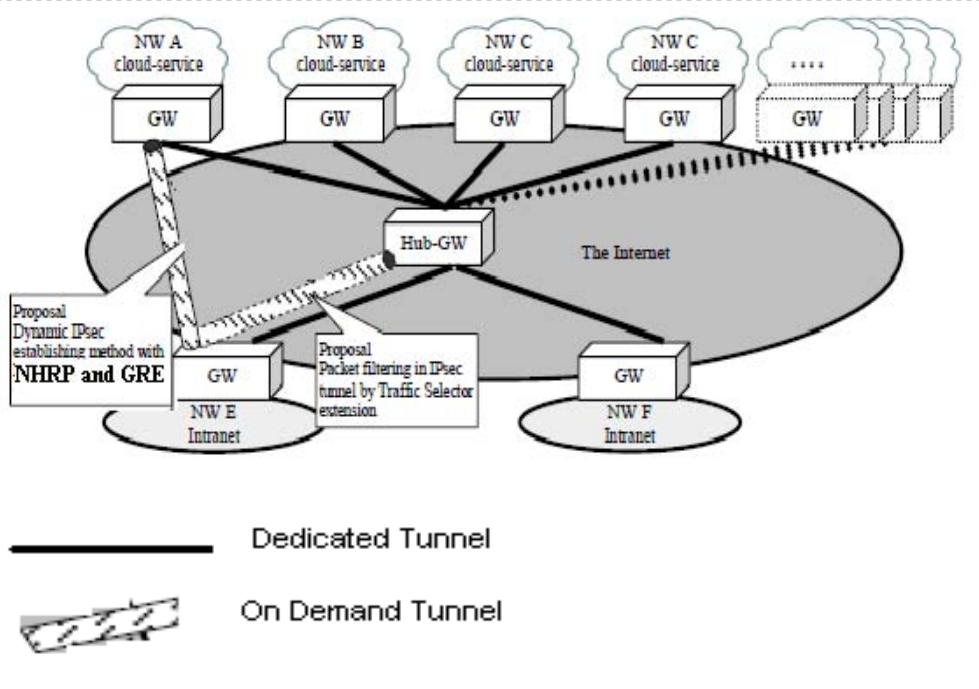
\includegraphics[height=5.5cm]{./pics/inter_cloud_architecture.png}
	\caption{Architecture proposé pour les communications inter-cloud \cite{archi_inter}}
	\label{label-image4}
\end{figure}

En conclusion, l'architecture proposé, appelé Dynamic Multipoint VPN, permet aux utilisateurs (ici, les fournisseurs de cloud) de mieux adapter les tunnels IPSecVPN en combinant le chiffrement d'IPSec, des tunnels GRE (\gls{GRE}) et le protocole NHRP. Les différents problèmes rencontrés dans les autres topologies IPSec VPN, Full-Mesh et Hub-and-Spoke, sont résolues avec les solutions proposées par cette architecture (voir \ref{label-image8}).

\begin{figure}[h]
	\center
	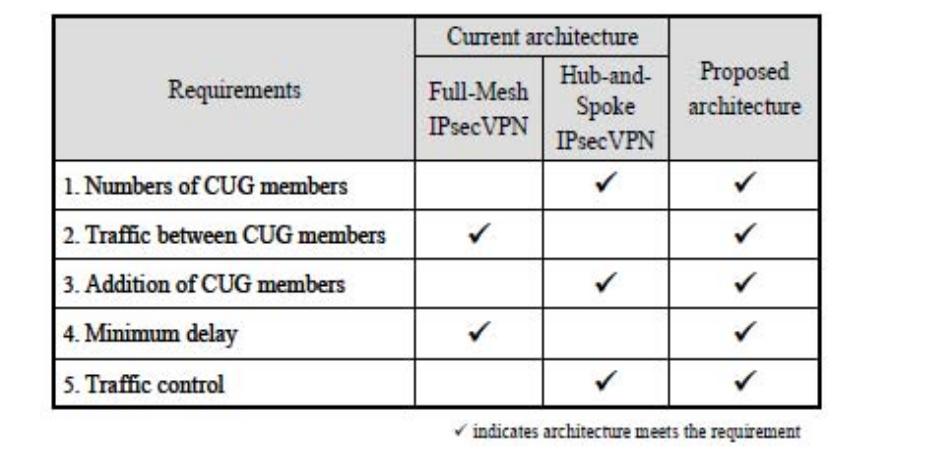
\includegraphics[height=5.5cm]{./pics/comparative_archi_inter_cloud.png}
	\caption{Comparaison des architectures IPSec VPN \cite{archi_inter}}
	\label{label-image8}
\end{figure}

Le cloud implique de nouveaux problèmes du à l'utilisation de l'architecture \textit{multi-tenant}. Une VM peut être corrompue et peut agir de manière malveillante. Un hôte interne du réseau est alors infecté et cible alors les machines du cloud. On parle alors d'une attaque interne impliquant les communications intra-cloud.
La deuxième partie du problème est donc de pouvoir sécuriser le cloud de possibles attaques internes. La démonstration de ce type d'attaque a été démontrée lors de la conférence
DefCon 18 par Bryan et Anderson (\cite{faiblesse_cloud}). Une attaque DDoS a été mise en place depuis le cloud EC2 d'Amazon et ils ciblaient une autre machine virtuelle, sur le même réseau.

\section{Communications intra-cloud}\label{sec:intra_cloud}

Aujourd'hui, les solutions actuelles, mises en place dans les cloud pour le sécuriser, utilisent des firewalls, des IDS et des IPS. Dans cette partie, nous allons tenter de proposer une solution performante en se basant sur le papier de Mazhar et al \cite{security_cloud_survey}. De plus, on ajoutera que le CSA (\cite{security_guidelines}) recommande l'utilisation de combinaisons de différents \gls{LAN} virtuels, d'IDS, d'IPS et d'un firewall afin de protéger les données en transit dans le cloud. 

\subsection{Solutions NIDS pour le cloud}

\subsubsection{SnortFlow}
\ag{Trop d'itemize}

\textit{SnortFlow} \cite{snortflow} est une solution proposée visant à améliorer les performances de \textit{Snort}. \textit{Snort} est un NIDS (Network IDS) orienté IDS/IPS : ce sont des solutions permettant de surveiller en temps réel un système et de détecter des activités suspectes violant la politique de sécurité du système. \textit{Snort} permet d'analyser le trafic en temps réel et enregistrer les paquets (log) au-dessus du protocole IP. Mais, les services proposées ne s'arrêtent pas là : 
recherche et correspondance de contenu, inhiber les \gls{prises d'empreintes} de la pile TCP/IP, dépassement de \textit{buffer}, scans, attaque CGI (Common Gateway Interface), sondes SMB (Server Message Block).
\textit{Snort} propose trois modes d'action du NIDS : le mode \textit{Sniffer} lit les paquets et les affiche, le mode \textit{Packet Logger} permet d'obtenir une log des paquets sur le disque et enfin, le mode \textit{Network Intrusion Detection System} qui gère le trafic et l'analyse avec les règles fixées par l'administrateur. Toutefois, le trafic ne doit pas être crypté, sinon le NIDS n'est plus capable de l'analyser.
Le fonctionnement de \textit{Snortflow} se base sur \textit{Snort} en ajoutant les fonctionnalités d'\textit{\gls{OpenFlow}}. \textit{OpenFlow} présente une nouvelle architecture pour fournir un environnement de réseau virtuel. L'idée sous-jacente est la séparation physique des plans de contrôle et de données. C'est la raison pour laquelle différents éléments exécutent la procédure de transfert de paquets (plan de données) et la procédure de contrôle de réseau (plan de contrôle). Le transfert est effectué grâce à une table de transfert partagée qui représente le plan de données, tandis que tous les plans de contrôle sont centralisées dans un nœud appelé contrôleur ou \textit{Controller}, faisant fonctionner les applications qui contrôlent le réseau virtuel. Ce contrôleur est un élément central du réseau. Il peut communiquer avec tous les nœuds pour configurer les tables de flux. Il travaille comme une interface entre les applications du réseau et les nœuds de transfert. Dans \textit{SnortFlow}, \textit{OpenFlow} est associé à \gls{POX}. Chaque plan de contrôle est composé d'un jeu d'application tournant sur POX. C'est la raison pour laquelle, dans \textit{OpenFlow}, un réseau virtuel est défini par son plan de contrôle, qui est un jeu d'applications fonctionnant sur le contrôleur, et par ses flux associés, provenant du \textit{Cloud Cluster} (voir \ref{label-image5}).

De plus, \textit{SnortFlow} se repose sur \textit{gls{XenServer}}. Xen est un hyperviseur ou \textit{Virtual Machine Monitor} qui fonctionne sur des plate-formes matérielles standards. En plus du VMM, situé lui sur le matériel physique, l'architecture Xen est composée de plusieurs domaines tournant de manière simultanée sur l'hyperviseur, appelés machines virtuelles. Chaque machine virtuelle peut avoir son propre système d'exploitation et ses applications. Le VMM contrôle l'accès au matériel des domaines multiples et gère le partage des ressources des différents domaines. Il existe deux types de domaines :
Le domaine 0, abrégé Dom0, est le domaine de gestion appartenant au domaine administratif du cloud. Le domaine, abrégé DomU, est le domaine hôte des VMs des utilisateurs.
Le Dom0 a des privilèges spéciaux comparé aux DomU et dispose, par exemple, d'un accès total au matériel de la machine physique. Les DomU possèdent des pilotes virtuels et opèrent comme s'ils pouvaient directement accéder au matériel. Cependant, ces pilotes virtuels communiquent avec le Dom0 afin d'avoir accès au matériel physique.
Donc, toutes les ressources de DomU sont gérés par Dom0, mais c'est \textit{OpenFlow Switch} (OFS) qui permet l'interconnexion les ressources sur différents serveurs clouds dans \textit{SnortFlow}. La communication entre les VMs doit donc obligatoirement passer par l'OVS, donc toutes les communications entre VMs sont analysés par le \textit{SnortFlow Agent} comme on peut le constater sur la figure \ref{label-image5}.
Le composant permettant de gérer et vérifier la sécurité du réseau est la partie \textit{SnortFlow Server}, car les communications analysées par \textit{SnortFlow Agent}  envoient des alertes lorsqu'un incident de sécurité apparaît tel qu'une violation de la politique de sécurité ou des données douteuses sont échangées. \textit{SnortFlow daemon} permet de collecter toutes les informations des alertes envoyées du \textit{SnortFlow Agent} et les envoyées à l'\textit{alert interpreter}. Ce dernier va analyser toutes les alertes et cibler les trafics suspects repérés. Le \textit{rules generator} va alors générer les règles qui vont être injectés dans le dispositif \textit{OpenFlow} où les nouvelles règles seront appliquées au réseau afin de ne plus laisser passer les trafics suspects repérés auparavant. Ces règles seront injectées dans une table appelés \textit{Flow Table}. Cependant, les faux positifs présents dans l'\textit{alert interpreter} sont nombreux et l'un des défis de \textit{SnortFlow} et des IDS en général est de minimiser au maximum l'apparition de ces faux positifs. Pour terminer, \textit{SnortFlow} propose une dernière fonctionnalité, appelé \textit{Network Reconfiguration}. Cette fonctionnalité va finaliser le processus des systèmes IPS. Elle octroie la possibilité de reconfigurer les caractéristiques du réseau tels que les paramètres de qualité de service ou encore la topologie. En ajoutant SDN au système des réseaux virtuels du cloud, cette fonctionnalité permet notamment d'appliquer des changements pour construire les contre-mesures des systèmes IPS dans les réseaux virtuels. En conclusion, lorsqu'une anomalie est détecté, le cloud va se défendre et mettre à jour ses données en enclenchant différents mécanismes.

\begin{figure}[h]
	\center
	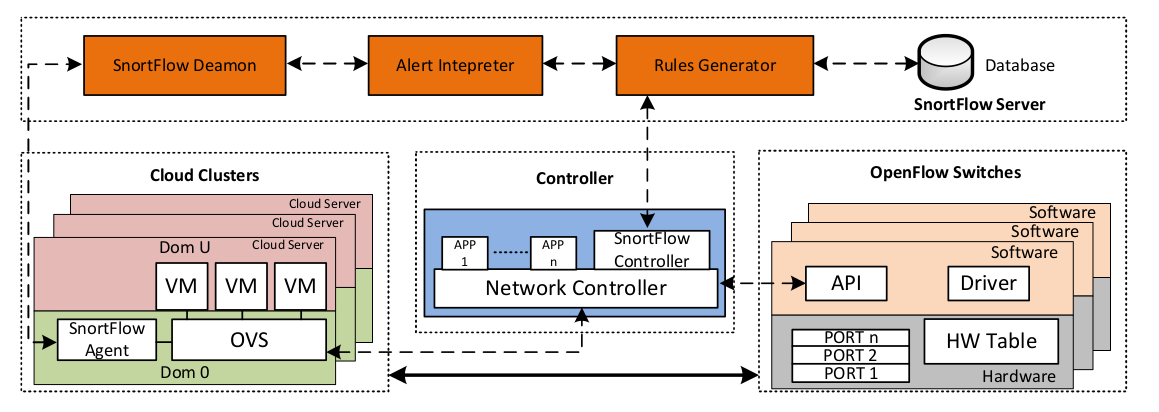
\includegraphics[height=5.5cm]{./pics/snortflow.png}
	\caption{Schéma fonctionnel de Snortflow [\cite{snortflow}]}
	\label{label-image5}
\end{figure}


\subsubsection{SDNIPS}

SDNIPS \cite{sdnips} est une solution reprenant tous les concepts de \textit{SnortFlow} en tentant de répondre à certains paramètres non présents, d'après les auteurs de SDNIPS, dans \textit{SnortFlow}  tels que : l'établissement d'un IDS efficace basé sur SDN et d'une architecture réseau permettant aux mécanismes défensifs des IDS/IPS d'être plus efficace. En effet, le fonctionnement de \textit{SnortFlow} est repris, ainsi que la majorité des composants utilisés (\textit{OpenFlow}, \textit{XenServer}), comme on peut le constater sur la figure \ref{label-image9}.

\begin{figure}[h]
	\center
	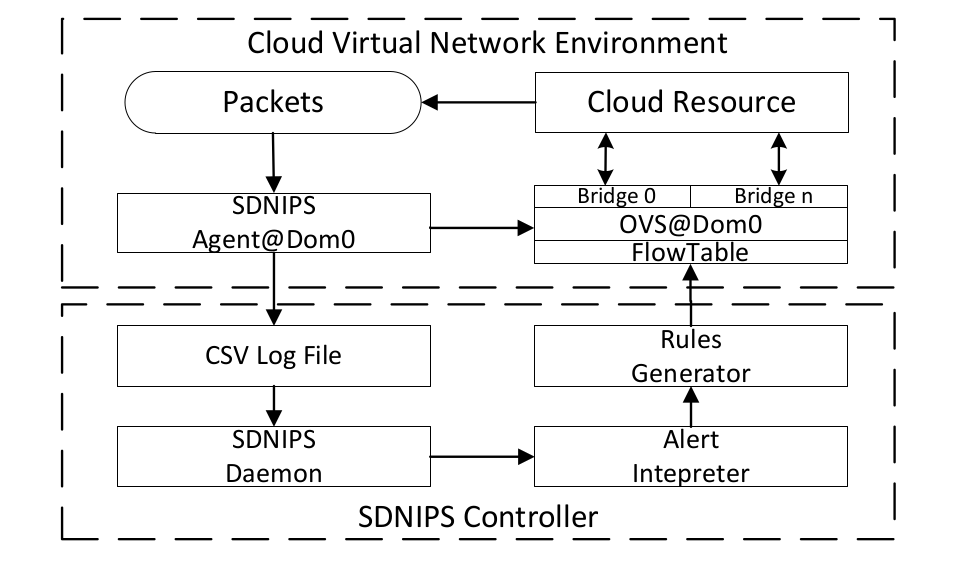
\includegraphics[height=5.5cm]{./pics/SDNIPS_fonctionnement.png}
	\caption{Fonctionnement de SDNIPS \cite{sdnips}}
	\label{label-image9}
\end{figure}

La principale différence entre les deux NIDS se traduit par une différence d'architecture. La figure \ref{label-image6} permet de visualiser l'architecture proposée par SDNIPS. \textit{Open vSwitch} est le \textit{switch} \textit{OpenFlow} et se compose de deux éléments dans l'espace utilisateur : \textit{ovsdb-server} et \textit{ovs-switchd}. Une des principales différences proposées est le déploiement direct de \textit{Snort} dans Dom0. Dom0 permet la détection et le traitement des paquets. En injectant \textit{Snort} dans Dom0, la détection des chemins virtuels vers les \textit{Virtual Interface} (VIF) s'effectue nativement dans OVS et offre une meilleure performance, car \textit{Snort} analyse et gère tous les réseaux virtuels dans le domaine privilégié.

\begin{figure}[h]
	\center
	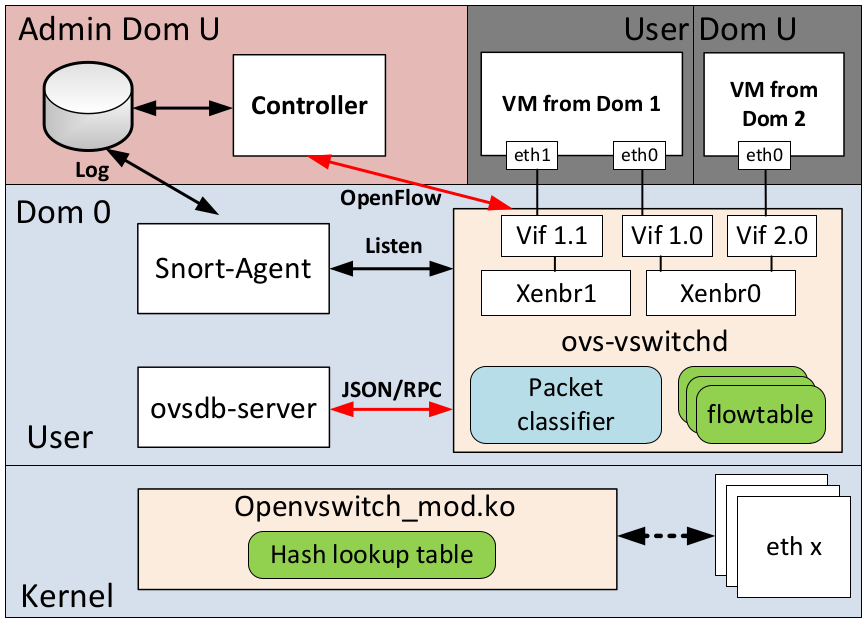
\includegraphics[height=5.5cm]{./pics/SDNIPS_architecture.png}
	\caption{Architecture de SDNIPS \cite{sdnips}}
	\label{label-image6}
\end{figure}


\subsubsection{Comparaison de Snortflow et SDNIPS}

\textit{SnortFlow} et SDNIPS sont tous les deux des systèmes IPS/IDS basés sur SDN générant dynamiquement des contre-mesures contre des attaques sur le réseau. 
Cependant, la faiblesse du papier de \textit{SnortFlow} est son manque d'évaluation et de comparaison. Les comparaisons effectuées n'apportent pas d'informations supplémentaires sur l'efficacité de \textit{SnortFlow}. Au contraire, SDNIPS apporte une comparaison entre le NIDS proposé et l'IPS "traditionnel" (\textit{Snort}/IPTables). Pour cette comparaison, ils ont inondé le réseau d'attaque DoS et ICMP. Il apparaît que SDNIPS détecte tous les paquets malveillants jusqu'à une limite de 15 000 paquets par seconde. L'IPS "traditionnel", lui, ne permet pas de détecter tous les paquets pendant une courte période et les auteurs notent que seuls 13,72\% des paquets ICMP sont détectés comme malveillants. On constate donc une différence importante de performance entre les deux outils. SDNIPS renforce la sécurité du cloud en détectant les anomalies, qu'elles soient nombreuses ou non. Ce type de comparaison est absente du papier présentant \textit{SnortFlow}. En conclusion, les deux papiers présentent des solutions similaires, mais l'absence d'une réelle évaluation de \textit{SnortFlow} justifie la préférence de mettre en avant SDNIPS comme NIDS dans ce rapport.

\begin{figure}[h]
	\center
	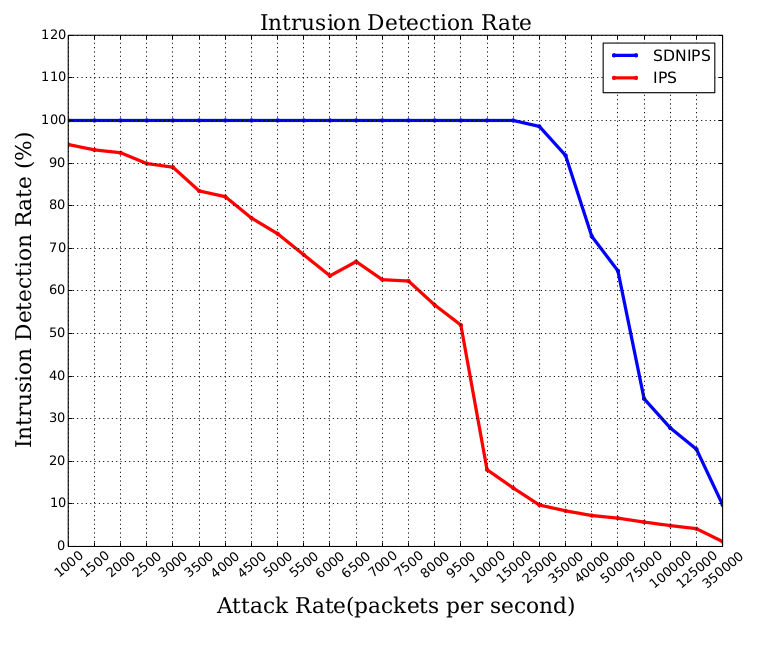
\includegraphics[height=6.5cm, width=10.5cm]{./pics/performance_SDNIPS.png}
	\caption{Évaluation du taux de détection d'intrusion entre un Snort/IPTable et SDNIPS \cite{sdnips}}
	\label{label-image10}
\end{figure}

\subsection{Firewall avec arbre de règle}
Pour conclure sur la sécurité des échanges intra-cloud, on ne pourra pas se passer d'un \textit{firewall}. La solution proposée par Xiangjian He et al. propose un \textit{firewall} sécurisé et performant. Il apparaît différent des \textit{firewalls} traditionnels, car il fonctionne via un arbre de règles et non pas une liste de règles (respectivement, \textit{Tree-rule} et \textit{Listed-rule}). Il propose un arbre et un ensemble de règles hiérarchiques, apparu dans les manuels de \textit{Cisco Services Switch} (CSS). Les \textit{Listed-rule firewall} apparaissent limité, car ce type de \textit{firewall} pose des problèmes de performance, de sécurité, mais également une difficulté à exploiter correctement ce type de \textit{firewall}. Dans ce papier, Xiangjian He et al. nous démontrent les différentes failles d'un \textit{Listed-rule firewall}. En premier lieu, la présence de \textit{shadowed rule} qui est l'une des grandes failles, car c'est une règle qui ne correspond à aucune entrée et pouvant créer ainsi des problèmes de sécurité et de performance. Autre inconvénient, les changement des positions des règles (dans le but d'affecter une règle plutôt qu'une autre pour un paquet) peut engendrer la modification de la politique de sécurité du \textit{firewall} et des failles de sécurité peuvent apparaître. De plus, des règles redondantes sont possibles et peuvent impacter la performance d'un \textit{firewall}. Un autre point négatif est la configuration d'un \textit{Listed-rule firewall}. En effet, un administrateur réseau a le devoir de localiser les plus grosses adresses réseaux aux plus petites (\textit{difficult to use}). Et enfin, les recherches séquentielles (ici recherche séquentielle des règles) pose des problèmes de rapidité et de performance.

La figure \ref{label-image7} permet de visualiser la forme du \textit{firewall} présenté dans le papier de Xiangjian He et al. Le \textit{firewall} lit les données contenues dans l'en-tête des paquets et va comparer les informations du paquet avec les règles des différents nœuds. On peut constater, sur la figure \ref{label-image7}, que à chaque nœud, des attributs différents sont comparés (Destination IP, Destination Port, Source IP). On peut donc spécifier une action spécifique pour certains paquets ou certains utilisateurs. De plus, les attributs présentés sont des exemples, on peut également travailler avec d'autres attributs ou bien même interchanger la place des différents attributs, c'est-à-dire placer la \textit{Destination Port} dans le premier nœud et la \textit{Destination IP} dans le deuxième nœud. Ce \textit{Tree-rule firewall} résout tous les problèmes posés par un \textit{Listed-rule firewall}. En effet, le \textit{firewall} proposé ne pose plus de problèmes de sécurité : les utilisateurs n'ont plus besoin d'effectuer des changements de position des règles et les \textit{shadowed rule} et les règles redondantes n'existent pas dans ce type de \textit{firewall}. Les paquets reçus passent les différents nœuds et suivent un chemin. Si aucun chemin n'est trouvé pour un paquet reçu, c'est-à-dire qu'il ne \textit{match} pas avec une règle contenue dans les nœuds pour un certain attribut, il est alors supprimé(\textit{Deny}). Sinon, on affecte une action spécifique (\textit{Accept}). Ensuite, l'exploitation et la configuration d'un \textit{Tree-rule firewall} est facile, il suffit d'intégrer les différentes informations dans les différentes colonnes des nœuds. Enfin, la complexité d'un arbre de règle est bien moins coûteuse qu'une liste de règles. Selon les auteurs, cette comparaison revient à comparer un arbre binaire de recherche et une recherche linéaire. 

\begin{figure}[h]
	\center
	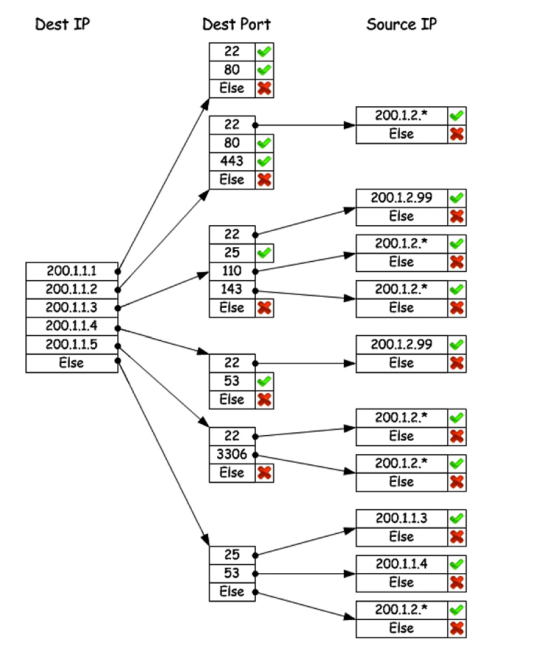
\includegraphics[height=8.5cm,width=11cm]{./pics/tree_rule_firewall.png}
	\caption{Structure d'un \textit{Tree-rule firewall} \cite{tree_rule_firewall}}
	\label{label-image7}
\end{figure}

De plus, IPTables apporte la plupart des fonctionnalités de base d'un \textit{firewall} (filtrage dynamique, translation de port et d'adresse, filtrage au niveau 2), mais lorsque le nombre de règles commence à être très grand, IPTables n'est plus capable d'apporter des performances satisfaisantes : moins de la moitié des règles sont atteintes avec IPTables quand le nombre de règles est de 5000. De plus, le CPU approche les 100\% d'utilisation. \textit{Tree-rule firewall} apporte toujours une excellente performance, malgré un nombre de règle important. Enfin, le CPU n'atteint même pas les 5\% d'utilisation. On peut donc affirmer que les performances du \textit{Tree-rule firewall} sont largement supérieur à IPTables. 
\newline
Pour conclure sur ce \textit{Tree-rule firewall}, les auteurs proposent  l'utilisation du \textit{firewall} sur un environnement cloud et proposent une comparaison entre différents \textit{firewall}. On constate via la figure \ref{label-image11} que le \textit{Tree-rule firewall} apporte des performances supplémentaires par rapport aux autres \textit{firewall}. La sécurité et les performances apportées par le \textit{Tree-rule firewall} sont importantes et vérifiées par les différentes comparaisons effectuées dans ce papier.

\begin{figure}[h]
	\center
	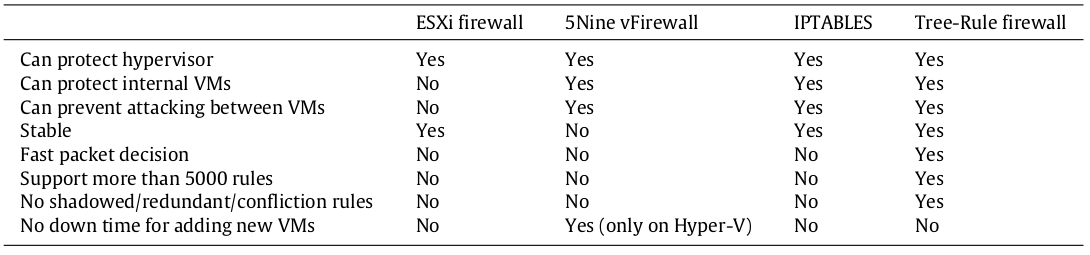
\includegraphics[height=3.5cm,width=15cm]{./pics/comparatif_firewall.png}
	\caption{Comparaison des fonctionnalités de différents\textit{firewall} dans un environnement cloud \cite{tree_rule_firewall}}
	\label{label-image11}
\end{figure}
